% Options for packages loaded elsewhere
\PassOptionsToPackage{unicode}{hyperref}
\PassOptionsToPackage{hyphens}{url}
%
\documentclass[
]{article}
\usepackage{amsmath,amssymb}
\usepackage{iftex}
\ifPDFTeX
  \usepackage[T1]{fontenc}
  \usepackage[utf8]{inputenc}
  \usepackage{textcomp} % provide euro and other symbols
\else % if luatex or xetex
  \usepackage{unicode-math} % this also loads fontspec
  \defaultfontfeatures{Scale=MatchLowercase}
  \defaultfontfeatures[\rmfamily]{Ligatures=TeX,Scale=1}
\fi
\usepackage{lmodern}
\ifPDFTeX\else
  % xetex/luatex font selection
\fi
% Use upquote if available, for straight quotes in verbatim environments
\IfFileExists{upquote.sty}{\usepackage{upquote}}{}
\IfFileExists{microtype.sty}{% use microtype if available
  \usepackage[]{microtype}
  \UseMicrotypeSet[protrusion]{basicmath} % disable protrusion for tt fonts
}{}
\makeatletter
\@ifundefined{KOMAClassName}{% if non-KOMA class
  \IfFileExists{parskip.sty}{%
    \usepackage{parskip}
  }{% else
    \setlength{\parindent}{0pt}
    \setlength{\parskip}{6pt plus 2pt minus 1pt}}
}{% if KOMA class
  \KOMAoptions{parskip=half}}
\makeatother
\usepackage{xcolor}
\usepackage{color}
\usepackage{fancyvrb}
\newcommand{\VerbBar}{|}
\newcommand{\VERB}{\Verb[commandchars=\\\{\}]}
\DefineVerbatimEnvironment{Highlighting}{Verbatim}{commandchars=\\\{\}}
% Add ',fontsize=\small' for more characters per line
\newenvironment{Shaded}{}{}
\newcommand{\AlertTok}[1]{\textcolor[rgb]{1.00,0.00,0.00}{\textbf{#1}}}
\newcommand{\AnnotationTok}[1]{\textcolor[rgb]{0.38,0.63,0.69}{\textbf{\textit{#1}}}}
\newcommand{\AttributeTok}[1]{\textcolor[rgb]{0.49,0.56,0.16}{#1}}
\newcommand{\BaseNTok}[1]{\textcolor[rgb]{0.25,0.63,0.44}{#1}}
\newcommand{\BuiltInTok}[1]{\textcolor[rgb]{0.00,0.50,0.00}{#1}}
\newcommand{\CharTok}[1]{\textcolor[rgb]{0.25,0.44,0.63}{#1}}
\newcommand{\CommentTok}[1]{\textcolor[rgb]{0.38,0.63,0.69}{\textit{#1}}}
\newcommand{\CommentVarTok}[1]{\textcolor[rgb]{0.38,0.63,0.69}{\textbf{\textit{#1}}}}
\newcommand{\ConstantTok}[1]{\textcolor[rgb]{0.53,0.00,0.00}{#1}}
\newcommand{\ControlFlowTok}[1]{\textcolor[rgb]{0.00,0.44,0.13}{\textbf{#1}}}
\newcommand{\DataTypeTok}[1]{\textcolor[rgb]{0.56,0.13,0.00}{#1}}
\newcommand{\DecValTok}[1]{\textcolor[rgb]{0.25,0.63,0.44}{#1}}
\newcommand{\DocumentationTok}[1]{\textcolor[rgb]{0.73,0.13,0.13}{\textit{#1}}}
\newcommand{\ErrorTok}[1]{\textcolor[rgb]{1.00,0.00,0.00}{\textbf{#1}}}
\newcommand{\ExtensionTok}[1]{#1}
\newcommand{\FloatTok}[1]{\textcolor[rgb]{0.25,0.63,0.44}{#1}}
\newcommand{\FunctionTok}[1]{\textcolor[rgb]{0.02,0.16,0.49}{#1}}
\newcommand{\ImportTok}[1]{\textcolor[rgb]{0.00,0.50,0.00}{\textbf{#1}}}
\newcommand{\InformationTok}[1]{\textcolor[rgb]{0.38,0.63,0.69}{\textbf{\textit{#1}}}}
\newcommand{\KeywordTok}[1]{\textcolor[rgb]{0.00,0.44,0.13}{\textbf{#1}}}
\newcommand{\NormalTok}[1]{#1}
\newcommand{\OperatorTok}[1]{\textcolor[rgb]{0.40,0.40,0.40}{#1}}
\newcommand{\OtherTok}[1]{\textcolor[rgb]{0.00,0.44,0.13}{#1}}
\newcommand{\PreprocessorTok}[1]{\textcolor[rgb]{0.74,0.48,0.00}{#1}}
\newcommand{\RegionMarkerTok}[1]{#1}
\newcommand{\SpecialCharTok}[1]{\textcolor[rgb]{0.25,0.44,0.63}{#1}}
\newcommand{\SpecialStringTok}[1]{\textcolor[rgb]{0.73,0.40,0.53}{#1}}
\newcommand{\StringTok}[1]{\textcolor[rgb]{0.25,0.44,0.63}{#1}}
\newcommand{\VariableTok}[1]{\textcolor[rgb]{0.10,0.09,0.49}{#1}}
\newcommand{\VerbatimStringTok}[1]{\textcolor[rgb]{0.25,0.44,0.63}{#1}}
\newcommand{\WarningTok}[1]{\textcolor[rgb]{0.38,0.63,0.69}{\textbf{\textit{#1}}}}
\usepackage{longtable,booktabs,array}
\usepackage{calc} % for calculating minipage widths
% Correct order of tables after \paragraph or \subparagraph
\usepackage{etoolbox}
\makeatletter
\patchcmd\longtable{\par}{\if@noskipsec\mbox{}\fi\par}{}{}
\makeatother
% Allow footnotes in longtable head/foot
\IfFileExists{footnotehyper.sty}{\usepackage{footnotehyper}}{\usepackage{footnote}}
\makesavenoteenv{longtable}
\usepackage{graphicx}
\makeatletter
\def\maxwidth{\ifdim\Gin@nat@width>\linewidth\linewidth\else\Gin@nat@width\fi}
\def\maxheight{\ifdim\Gin@nat@height>\textheight\textheight\else\Gin@nat@height\fi}
\makeatother
% Scale images if necessary, so that they will not overflow the page
% margins by default, and it is still possible to overwrite the defaults
% using explicit options in \includegraphics[width, height, ...]{}
\setkeys{Gin}{width=\maxwidth,height=\maxheight,keepaspectratio}
% Set default figure placement to htbp
\makeatletter
\def\fps@figure{htbp}
\makeatother
\setlength{\emergencystretch}{3em} % prevent overfull lines
\providecommand{\tightlist}{%
  \setlength{\itemsep}{0pt}\setlength{\parskip}{0pt}}
\setcounter{secnumdepth}{-\maxdimen} % remove section numbering
\ifLuaTeX
  \usepackage{selnolig}  % disable illegal ligatures
\fi
\usepackage{bookmark}
\IfFileExists{xurl.sty}{\usepackage{xurl}}{} % add URL line breaks if available
\urlstyle{same}
\hypersetup{
  pdftitle={Indice},
  hidelinks,
  pdfcreator={LaTeX via pandoc}}

\title{Indice}
\author{}
\date{}

\begin{document}
\maketitle

\begin{enumerate}
\tightlist
\item
  Introduzione
\item
  Specifica dei requisiti

  \begin{enumerate}
  \tightlist
  \item
    Requisiti funzionali
  \item
    Requisiti non funzionali
  \end{enumerate}
\item
  Descrizione del progetto
\item
  UML

  \begin{enumerate}
  \tightlist
  \item
    Use case diagram
  \item
    Activity diagram

    \begin{enumerate}
    \tightlist
    \item
      Activity diagram della dispensa
    \item
      Activity diagram della lista della spesa
    \item
      Activity diagram delle ricette
    \end{enumerate}
  \item
    State diagram

    \begin{enumerate}
    \tightlist
    \item
      State diagram della ricetta
    \item
      State diagram della lista della spesa
    \end{enumerate}
  \item
    Class diagram
  \item
    Sequence diagram

    \begin{enumerate}
    \tightlist
    \item
      Sequence diagram della dispensa
    \item
      Sequence diagram della lista della spesa
    \item
      Sequence diagram delle ricette
    \end{enumerate}
  \end{enumerate}
\item
  Design Pattern

  \begin{enumerate}
  \tightlist
  \item
    Factory
  \item
    Iterator
  \item
    Observer
  \item
    Singleton
  \item
    Decorator
  \end{enumerate}
\item
  ORM\\
  1. Vantaggi\\
  2. Svantaggi\\
  3. Stress tests
\end{enumerate}

\subsection{1. Introduzione}\label{introduzione}

Expiration Date è un\textquotesingle applicazione nata per permettere la
gestione completa di tutto ciò che riguarda i prodotti alimentari; con
essa è infatti possibile gestire gli aspetti relativi:

\begin{itemize}
\tightlist
\item
  alla lista della spesa (prodotti che si desidera acquistare)
\item
  alla dispensa (prodotti già posseduti)
\item
  alle ricette
\end{itemize}

\subsection{2. Specifica dei requisiti}\label{specifica-dei-requisiti}

Nelle sezioni seguenti verranno illustrati i principali requisiti che
l\textquotesingle applicazione si pone come obiettivo di soddisfare.

\subsubsection{2.1 Requisiti funzionali}\label{requisiti-funzionali}

Essi descrivono le funzionalità che il sistema deve offrire, intendendo
con questo sia le operazioni che l\textquotesingle applicazione svolge
sia le interazioni che la stessa ha con l\textquotesingle utente o con
altri sistemi esterni con cui si interfaccia.

\begin{longtable}[]{@{}ll@{}}
\toprule\noalign{}
RF01 & Aggiunta alimenti in dispensa \\
\midrule\noalign{}
\endhead
\bottomrule\noalign{}
\endlastfoot
Input & Dati alimento acquistato - nome alimento, data di scadenza,
quantità \\
Processo & Memorizzazione su lista e database degli alimenti \\
Output & Visualizzazione alimenti \\
\end{longtable}

~

\begin{longtable}[]{@{}ll@{}}
\toprule\noalign{}
RF01.1 & Generazione notifica scadenza alimento \\
\midrule\noalign{}
\endhead
\bottomrule\noalign{}
\endlastfoot
Input & Aggiunta di un prodotto alla dispensa \\
Processo & Si crea l'avviso su calendario relativo alla scadenza del
prodotto \\
Output & Aggiunta dell'avviso sul calendario dell'utente \\
\end{longtable}

~

\begin{longtable}[]{@{}ll@{}}
\toprule\noalign{}
RF02 & Rimozione alimenti in dispensa \\
\midrule\noalign{}
\endhead
\bottomrule\noalign{}
\endlastfoot
Input & click su pulsante ``delete'' \\
Processo & Eliminazione alimento dalla lista e dal database \\
Output & Visualizzazione lista aggiornata \\
\end{longtable}

~

\begin{longtable}[]{@{}ll@{}}
\toprule\noalign{}
RF02.1 & Rimozione avviso su calendario \\
\midrule\noalign{}
\endhead
\bottomrule\noalign{}
\endlastfoot
Input & Rimozione prodotto dalla dispensa \\
Processo & Cancellazione avviso su calendario \\
Output & Rimozione avviso su calendario \\
\end{longtable}

~

\begin{longtable}[]{@{}ll@{}}
\toprule\noalign{}
RF03 & Ordinamento prodotti dispensa per nome \\
\midrule\noalign{}
\endhead
\bottomrule\noalign{}
\endlastfoot
Input & Clic sulla colonna ``Product'' \\
Processo & Ordinamento prodotti in modo crescente o decrescente in base
al nome \\
Output & Visualizzazione prodotti ordinati \\
\end{longtable}

~

\begin{longtable}[]{@{}ll@{}}
\toprule\noalign{}
RF04 & Ordinamento prodotti dispensa per data di scadenza \\
\midrule\noalign{}
\endhead
\bottomrule\noalign{}
\endlastfoot
Input & Clic sulla colonna ``Expiration Date'' \\
Processo & Ordinamento prodotti in modo crescente o decrescente in base
alla data di scadenza \\
Output & Visualizzazione prodotti ordinati \\
\end{longtable}

~

\begin{longtable}[]{@{}ll@{}}
\toprule\noalign{}
RF05 & Modifica nome alimento in dispensa \\
\midrule\noalign{}
\endhead
\bottomrule\noalign{}
\endlastfoot
Input & Doppio clic sul nome alimento e inserimento nuovo nome \\
Processo & Aggiornamento nome alimento in memoria e in database \\
Output & Visualizzazione alimento con nome aggiornato \\
\end{longtable}

~

\begin{longtable}[]{@{}ll@{}}
\toprule\noalign{}
RF06 & Modifica dati alimento in dispensa \\
\midrule\noalign{}
\endhead
\bottomrule\noalign{}
\endlastfoot
Input & Doppio clic su data di scadenza e modifica dati \\
Processo & Si apre una nuova finestra che consente la modifica dei dati
dell'alimento; Aggiornamento dati alimento in memoria e in database \\
Output & Visualizzazione alimenti aggiornati \\
\end{longtable}

~

~

~

\begin{longtable}[]{@{}ll@{}}
\toprule\noalign{}
RF06.1 & Modifica avviso calendario \\
\midrule\noalign{}
\endhead
\bottomrule\noalign{}
\endlastfoot
Input & Modifica data di scadenza e/o nome prodotto \\
Processo & Aggiornamento data di scadenza e/o nome prodotto sul
calendario \\
Output & Visualizzazione calendario aggiornato \\
\end{longtable}

~

\begin{longtable}[]{@{}ll@{}}
\toprule\noalign{}
RF07 & Aggiunta alimenti in lista della spesa \\
\midrule\noalign{}
\endhead
\bottomrule\noalign{}
\endlastfoot
Input & Nome alimento da acquistare \\
Processo & Salvataggio su memoria e database della lista della spesa \\
Output & Visualizzazione shopping list \\
\end{longtable}

~

\begin{longtable}[]{@{}ll@{}}
\toprule\noalign{}
RF08 & Rimozione alimenti in lista della spesa \\
\midrule\noalign{}
\endhead
\bottomrule\noalign{}
\endlastfoot
Input & click su pulsante ``delete'' \\
Processo & Eliminazione alimento dalla lista e dal database della lista
della spesa \\
Output & Visualizzazione aggiornata lista della spesa \\
\end{longtable}

~

\begin{longtable}[]{@{}ll@{}}
\toprule\noalign{}
RF09 & Alimento in lista della spesa comprato \\
\midrule\noalign{}
\endhead
\bottomrule\noalign{}
\endlastfoot
Input & Utente clicca sulla checkbox che segnala l'acquisto di un
elemento nella lista della spesa \\
Processo & Viene azionata la stessa procedura che implementa il
requisito RF01 \\
Output & Visualizzazione alimenti e aggiornamento lista della spesa \\
\end{longtable}

~

\begin{longtable}[]{@{}ll@{}}
\toprule\noalign{}
RF10 & Pulizia lista della spesa \\
\midrule\noalign{}
\endhead
\bottomrule\noalign{}
\endlastfoot
Input & Click sul pulsante ``clear'' della shopping list \\
Processo & Rimozione dalla shopping list, sia in memoria che in
database, degli alimenti già acquistati \\
Output & Visualizzazione shopping list aggiornata \\
\end{longtable}

~

~

~

\begin{longtable}[]{@{}ll@{}}
\toprule\noalign{}
RF11 & Visualizzazione ricette memorizzate \\
\midrule\noalign{}
\endhead
\bottomrule\noalign{}
\endlastfoot
Input & Click sul pulsante ``Recipe'' nella dispensa e all'interno della
schermata ``Recipe'' attraverso le frecce di navigazione è possibile
passare da una ricetta alla successiva \\
Processo & Caricamento dal database delle ricette \\
Output & Visualizzazione ricette \\
\end{longtable}

~

\begin{longtable}[]{@{}ll@{}}
\toprule\noalign{}
RF12 & Aggiunta ricette \\
\midrule\noalign{}
\endhead
\bottomrule\noalign{}
\endlastfoot
Input & Click su pulsante ``Add'' e inserimento dati ricetta - titolo,
durata, numero porzioni, categoria, lista dei tag, lista ingredienti,
procedimento ricetta \\
Processo & Salvataggio su database e in memoria della ricetta \\
Output & Visualizzazione ricetta \\
\end{longtable}

~

\begin{longtable}[]{@{}ll@{}}
\toprule\noalign{}
RF13 & Modifica dati ricetta \\
\midrule\noalign{}
\endhead
\bottomrule\noalign{}
\endlastfoot
Input & Modifiche su dati ricetta \\
Processo & Salvataggio in memoria e database dei dati della ricetta
aggiornati \\
Output & Visualizzazione ricetta aggiornata \\
\end{longtable}

~

\begin{longtable}[]{@{}ll@{}}
\toprule\noalign{}
RF14 & Controllo disponibilità ingredienti \\
\midrule\noalign{}
\endhead
\bottomrule\noalign{}
\endlastfoot
Input & Visualizzazione ricetta o modifica della stessa \\
Processo & Confronto fra i prodotti in dispensa e gli ingredienti
necessari per la ricetta \\
Output & Visualizzazione ingredienti disponibili e non disponibili per
la ricetta attuale \\
\end{longtable}

~

\begin{longtable}[]{@{}ll@{}}
\toprule\noalign{}
RF15 & Eliminazione ricetta \\
\midrule\noalign{}
\endhead
\bottomrule\noalign{}
\endlastfoot
Input & Click sul pulsante ``Delete'' nella schermata delle ricette \\
Processo & Rimozione da memoria e database della ricetta attuale \\
Output & Visualizzazione di un'altra ricetta o aggiunta di una nuova
ricetta vuota se non ci sono più ricette \\
\end{longtable}

~

\begin{longtable}[]{@{}ll@{}}
\toprule\noalign{}
RF16 & Import ricette da file \\
\midrule\noalign{}
\endhead
\bottomrule\noalign{}
\endlastfoot
Input & File contenente una lista di ricette \\
Processo & Salvataggio in memoria e database dei dati della ricette sul
file importato \\
Output & Visualizzazione ricette importate \\
\end{longtable}

~

\begin{longtable}[]{@{}ll@{}}
\toprule\noalign{}
RF17 & Export ricette su file \\
\midrule\noalign{}
\endhead
\bottomrule\noalign{}
\endlastfoot
Input & Click su pulsante ``Export'' \\
Processo & Creazione di un file su cui sono memorizzate le ricette
presenti in database \\
Output & File con lista delle ricette \\
\end{longtable}

\subsubsection{2.2 Non funzionali}\label{non-funzionali}

Essi descrivono le caratteristiche che l\textquotesingle applicazione
deve avere che non sono direttamente collegate alle operazioni che
esegue.

\begin{longtable}[]{@{}ll@{}}
\toprule\noalign{}
RNF01 & Tempi di risposta \\
\midrule\noalign{}
\endhead
\bottomrule\noalign{}
\endlastfoot
Descrizione & Il software dovrà garantire tempi di risposta minimi per
tutte le operazioni, consentendo agli utenti di interagire con
l\textquotesingle applicazione in tempo reale \\
\end{longtable}

~

\begin{longtable}[]{@{}ll@{}}
\toprule\noalign{}
RNF02 & Database (salvataggio dei dati) \\
\midrule\noalign{}
\endhead
\bottomrule\noalign{}
\endlastfoot
Descrizione & L\textquotesingle applicazione dovrà utilizzare un sistema
di database affidabile e sicuro per garantire la persistenza dei dati
relativi ai prodotti nella dispensa, ai prodotti presenti nella lista
della spesa e alle ricette \\
\end{longtable}

~

\begin{longtable}[]{@{}ll@{}}
\toprule\noalign{}
RNF03 & Portabilità \\
\midrule\noalign{}
\endhead
\bottomrule\noalign{}
\endlastfoot
Descrizione & L\textquotesingle applicazione deve essere progettata in
modo da essere compatibile sia con i sistemi Android che iOS \\
\end{longtable}

~

\begin{longtable}[]{@{}ll@{}}
\toprule\noalign{}
RNF04 & Integrazione con servizi di terze parti \\
\midrule\noalign{}
\endhead
\bottomrule\noalign{}
\endlastfoot
Descrizione & Il sistema deve essere in grado di interagire con il
calendario predefinito dell\textquotesingle utente \\
\end{longtable}

\subsection{3. Descrizione del progetto}\label{descrizione-del-progetto}

Per questa descrizione si farà riferimento alla versione desktop
dell\textquotesingle applicazione.

Il software presenta due schermate principali:

\begin{itemize}
\tightlist
\item
  una per la gestione della dispensa e della lista della spesa
\item
  una per la gestione delle ricette
\end{itemize}

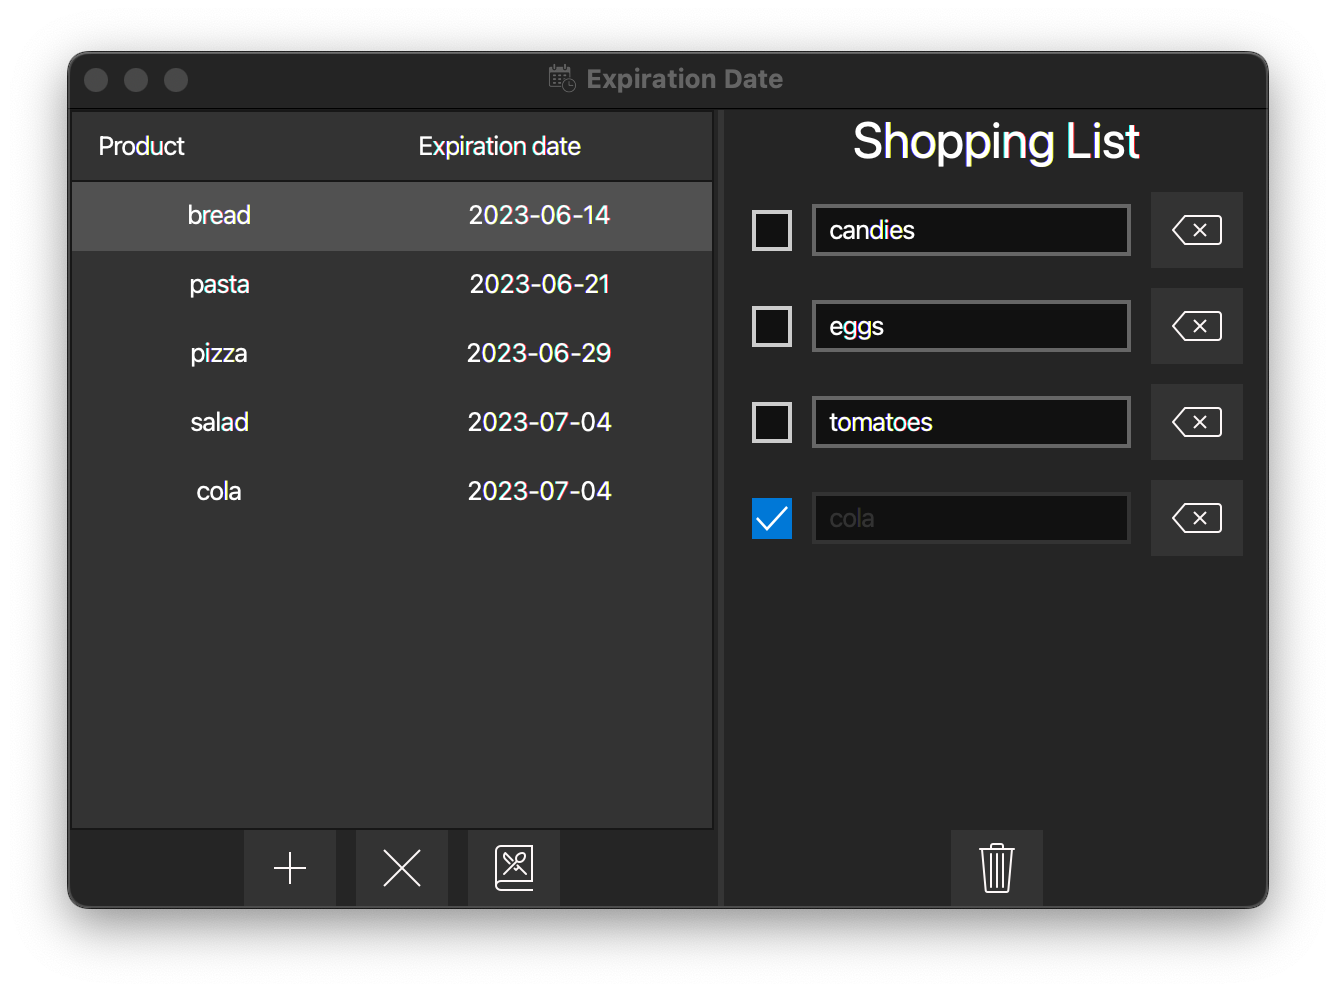
\includegraphics{/Users/saverionapolitano/Library/Mobile Documents/iCloud~md~obsidian/Documents/University/main-view.png}

La schermata per la gestione della dispensa e della lista della spesa si
divide in due parti:

\begin{itemize}
\tightlist
\item
  la parte di sinistra permette di aggiungere prodotti alla dispensa,
  eliminare prodotti dalla dispensa, modificare i dati di un prodotto o
  passare alla schermata delle ricette

  \begin{itemize}
  \tightlist
  \item
    Nel caso si desideri modificare i dati di un prodotto comparirà una
    schermata apposita per la modifica
  \end{itemize}
\end{itemize}

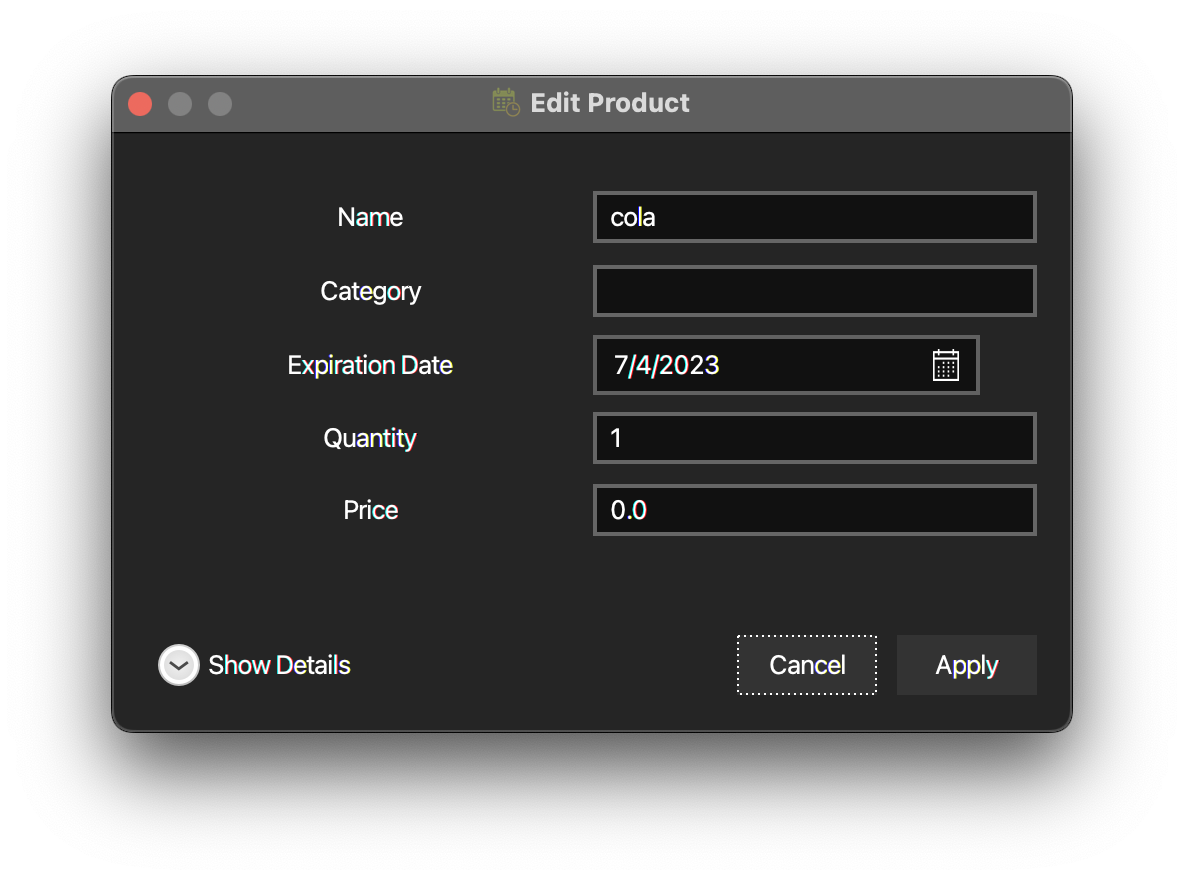
\includegraphics{/Users/saverionapolitano/Library/Mobile Documents/iCloud~md~obsidian/Documents/University/edit-product.png}

\begin{itemize}
\tightlist
\item
  la parte di destra permette di aggiungere prodotti alla lista della
  spesa, eliminare prodotti dalla lista della spesa, contrassegnare un
  prodotto della lista della spesa come "acquistato" (e aggiungerlo in
  automatico alla dispensa) e rimuovere tutti i prodotti contrassegnati
  come acquistati
\end{itemize}

La schermata per la gestione delle ricette permette di navigare tra le
ricette con le apposite frecce, aggiungere una ricetta, rimuovere una
ricetta, modificare i dati di una ricetta, importare ed esportare liste
di ricette.

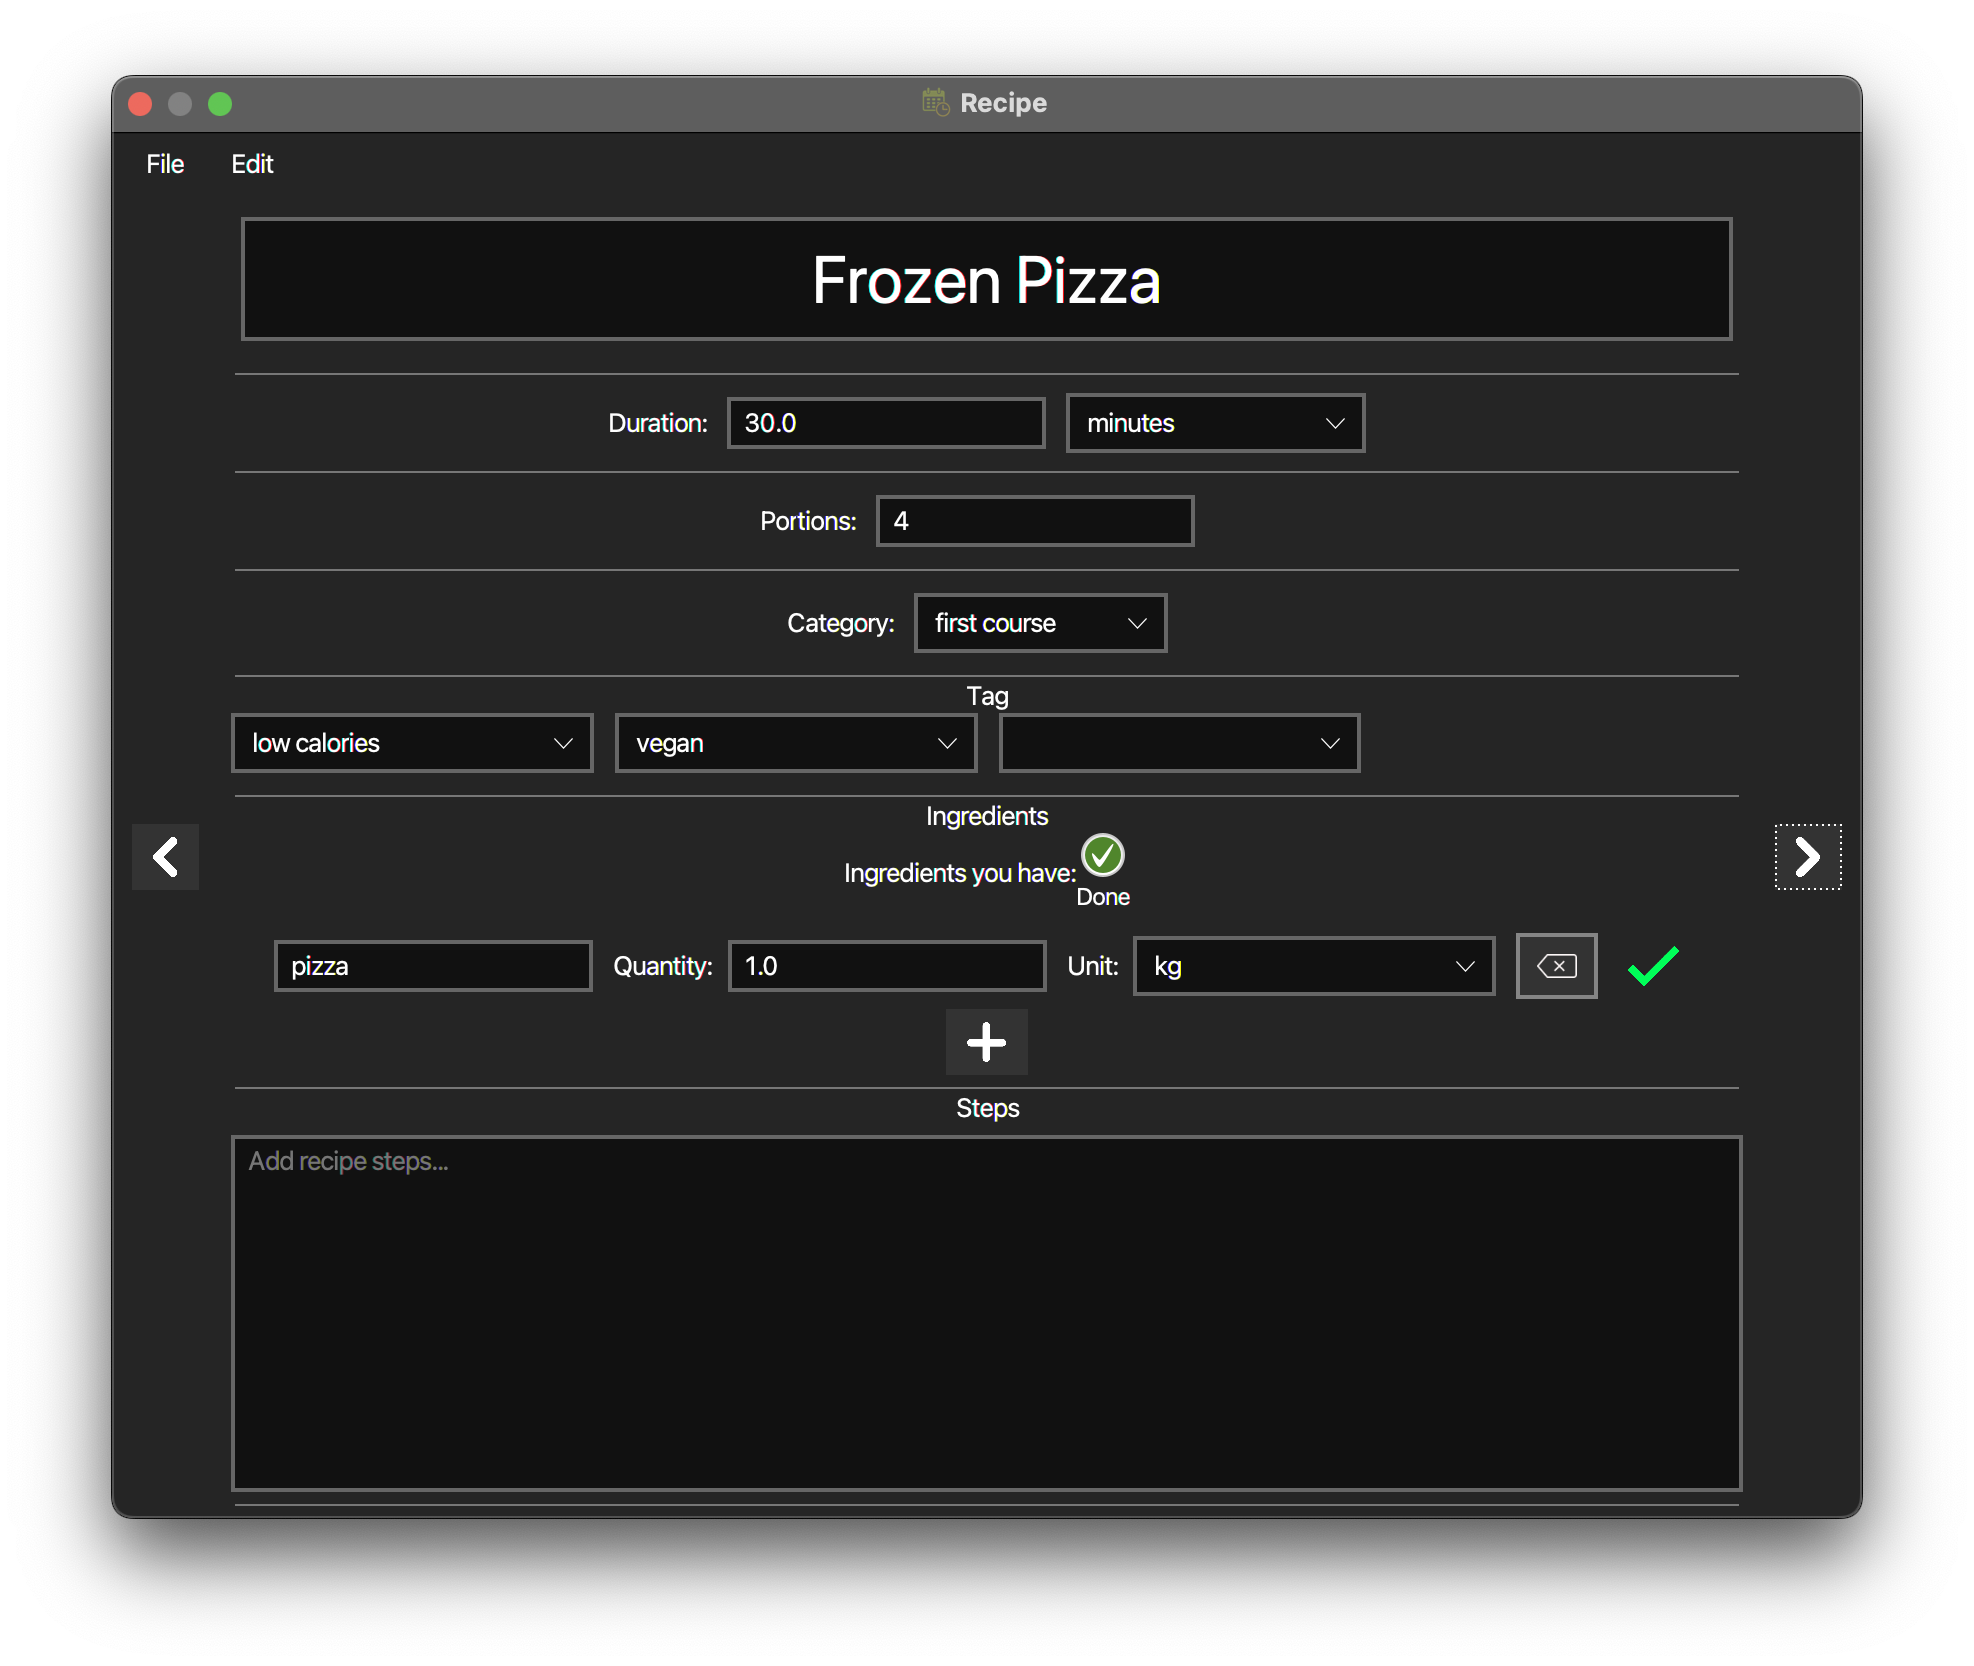
\includegraphics{/Users/saverionapolitano/Library/Mobile Documents/iCloud~md~obsidian/Documents/University/recipe-view.png}

\subsection{4. UML}\label{uml}

I diagrammi UML permettono di descrivere graficamente
l\textquotesingle applicazione sotto vari punti di vista, garantendo la
comprensione del funzionamento del software, delle esigenze che esso
soddisfa e delle relazioni che intercorrono fra i suoi componenti.

\subsubsection{4.1 Use case diagram}\label{use-case-diagram}

Lo use case diagram permette di identificare gli attori che
interagiscono col sistema e le attività che essi possono svolgere. Lo
scopo è descrivere le principali funzionalità del software.

\includegraphics{/Users/saverionapolitano/Library/Mobile Documents/iCloud~md~obsidian/Documents/University/UseCaseTesinaSperoFinale.png}

\subsubsection{4.2 Activity diagram}\label{activity-diagram}

L\textquotesingle activity diagram consente di specificare come il
sistema realizzerà le funzionalità mostrate nello use case. Lo scopo è
connettere tra loro azioni di alto livello per rappresentare un processo
che viene svolto nel sistema. Per una migliore comprensione del
funzionamento, nei diagrammi seguenti si è scelto di non modellare i
casi di errore del database e dell\textquotesingle interfaccia grafica.

\paragraph{4.2.1 Activity diagram della
dispensa}\label{activity-diagram-della-dispensa}

In questo diagramma viene mostrato il processo relativo
all\textquotesingle interazione fra l\textquotesingle utente e
l\textquotesingle applicazione per la gestione della dispensa.

\includegraphics{/Users/saverionapolitano/Library/Mobile Documents/iCloud~md~obsidian/Documents/University/ActivityDispensaTesinaSperoFinale.png}

\paragraph{4.2.2 Activity diagram della lista della
spesa}\label{activity-diagram-della-lista-della-spesa}

In questo diagramma viene mostrato il processo relativo
all\textquotesingle interazione fra l\textquotesingle utente e
l\textquotesingle applicazione per la gestione della lista della spesa.

\includegraphics{/Users/saverionapolitano/Library/Mobile Documents/iCloud~md~obsidian/Documents/University/ActivityListaSpesaTesinaSperoFinale.png}

\paragraph{4.2.3 Activity diagram delle
ricette}\label{activity-diagram-delle-ricette}

In questo diagramma viene mostrato il processo relativo
all\textquotesingle interazione fra l\textquotesingle utente e
l\textquotesingle applicazione per la gestione delle ricette, inclusa la
possibilità di importare ed esportare ricette.

\includegraphics{/Users/saverionapolitano/Library/Mobile Documents/iCloud~md~obsidian/Documents/University/ActivityRicetteTesinaSperoFinale.png}

\subsubsection{4.3 State diagram}\label{state-diagram}

Lo state diagram permette di modellare gli stati in cui si trova un
oggetto e gli eventi che causano le transizioni fra gli stati.

\paragraph{4.3.1 State diagram della
ricetta}\label{state-diagram-della-ricetta}

In questo diagramma vengono mostrati gli stati in cui si può trovare una
ricetta in base alla presenza, e alla disponibilità, degli ingredienti.

\includegraphics[width=5.20833in,height=\textheight]{/Users/saverionapolitano/Library/Mobile Documents/iCloud~md~obsidian/Documents/University/StateDiagramRicettaTesina.png}

\paragraph{4.3.2 State diagram della lista della
spesa}\label{state-diagram-della-lista-della-spesa}

In questo diagramma vengono mostrati gli stati in cui si può trovare un
prodotto presente nella lista della spesa.

\includegraphics[width=5.20833in,height=\textheight]{/Users/saverionapolitano/Library/Mobile Documents/iCloud~md~obsidian/Documents/University/StateListaSpesaSperoFinale.png}

\subsubsection{4.4 Class diagram}\label{class-diagram}

Il class diagram permette di descrivere i tipi di oggetti presenti nel
sistema e le relazioni statiche che intercorrono tra di essi. Esso
descrive inoltre gli attributi e i metodi di ogni classe, oltre ai
vincoli che si applicano nel collegamento tra gli oggetti.

\includegraphics{/Users/saverionapolitano/Library/Mobile Documents/iCloud~md~obsidian/Documents/University/IMG_44D526B57139-1.jpeg}

Per non complicare ulteriormente il diagramma si è scelto di non
rappresentare la parte relativa all\textquotesingle interfaccia grafica.
I design pattern applicati verranno spiegati nella sezione
corrispondente.

\subsubsection{4.5 Sequence diagram}\label{sequence-diagram}

Il sequence diagram serve per descrivere singoli scenari
dell\textquotesingle applicazioni. Lo scopo è mostrare come il sistema
svolge le proprie funzioni. Per una migliore comprensione del
funzionamento, nei diagrammi seguenti si è scelto di non modellare i
casi di errore del database e dell\textquotesingle interfaccia grafica.

\paragraph{4.5.1 Sequence diagram della
dispensa}\label{sequence-diagram-della-dispensa}

\includegraphics{/Users/saverionapolitano/Library/Mobile Documents/iCloud~md~obsidian/Documents/University/sequenceDispensaTesinaSperoFinale.png}

\paragraph{4.5.2 Sequence diagram della lista della
spesa}\label{sequence-diagram-della-lista-della-spesa}

\includegraphics{/Users/saverionapolitano/Library/Mobile Documents/iCloud~md~obsidian/Documents/University/sequenceListaSpesaTesinaSperoFinale-2.png}

\paragraph{4.5.3 Sequence diagram delle
ricette}\label{sequence-diagram-delle-ricette}

Si noti che, per evitare sovrapposizioni nel diagramma che ne avrebbero
resa più difficile la comprensione, il metodo
\texttt{creaRicettaVuota()} (che si limita a mostrare dei campi di testo
vuoti all\textquotesingle utente tramite l\textquotesingle interfaccia
grafica) non crea un oggetto di tipo Ricetta (come invece avviene nel
caso del metodo
\texttt{aggiungiRicetta(ingredienti,\ preparazione,\ porzioni,\ durata,\ tags)}
in cui la ricetta creata presenta valori non nulli nei propri
attributi).

\includegraphics[width=6.25in,height=\textheight]{/Users/saverionapolitano/Library/Mobile Documents/iCloud~md~obsidian/Documents/University/sequenceRicetteTesina.png}

\subsection{5. Design Pattern}\label{design-pattern}

\subsubsection{5.1 Factory}\label{factory}

Il design pattern Factory ha il compito di occuparsi della creazione dei
prodotti. L\textquotesingle utilizzo di questo design permette di
evitare di programmare verso le implementazioni concrete, favorendo la
programmazione verso le interfacce. Senza di esso, quando in futuro
dovranno essere apportare modifiche o estensioni, sarebbe necessario
riaprire il codice e cambiarlo di conseguenza (violando quindi
l\textquotesingle open-closed principle). Incapsulare la creazione dei
prodotti in una apposita classe permette di evitare questo scenario,
oltre a facilitare la manutenzione e l\textquotesingle aggiornamento
dell\textquotesingle applicazione: le modifiche sono infatti localizzate
unicamente nella classe Factory, mentre in mancanza di essa sarebbe
necessario cambiare manualmente tutti i punti del codice in cui
c\textquotesingle è un "new" di un prodotto. L\textquotesingle utilizzo
del design pattern Factory rispetta inoltre il dependency inversion
principle.

\begin{Shaded}
\begin{Highlighting}[]
\NormalTok{public abstract class Bevanda extends Prodotto\{  }
\NormalTok{    boolean zuccherata;  }
\NormalTok{    public Bevanda(String nome, LocalDate dataScadenza, int quantità, double prezzo, String categoria) \{  }
\NormalTok{       super(nome, dataScadenza, quantità, prezzo, categoria);  }
\NormalTok{    \}  }
\NormalTok{\}}

\NormalTok{public class Zuccherata extends Bevanda\{  }
  
\NormalTok{    public Zuccherata(String nome, LocalDate dataScadenza, int quantità, double prezzo, String categoria) \{  }
\NormalTok{       super(nome, dataScadenza, quantità, prezzo, categoria);   }
\NormalTok{       zuccherata = true;  }
\NormalTok{    \}}
\NormalTok{\}}

\NormalTok{public abstract class ProdottoFactory \{  }
\NormalTok{    public abstract Prodotto creaProdotto(String nome, LocalDate dataScadenza, int quantità, double prezzo, String categoria);  }
\NormalTok{\}}

\NormalTok{public class ConcreteProdottoFactory extends ProdottoFactory \{}
\NormalTok{    @Override}
\NormalTok{    public Prodotto creaProdotto(String nome, LocalDate dataScadenza, int quantità, double prezzo, String categoria) \{}
\NormalTok{        if("bevanda zuccherata".equals(categoria))\{}
\NormalTok{            return new Zuccherata(nome, dataScadenza, quantità, prezzo, categoria);}
\NormalTok{        \} else if("bevanda non zuccherata".equals(categoria))\{}
\NormalTok{            return new NonZuccherata(nome, dataScadenza, quantità, prezzo, categoria);}
\NormalTok{        \} else if("prodotto generico".equals(categoria))\{}
\NormalTok{            return new Generico(nome, dataScadenza, quantità, prezzo, categoria);}
\NormalTok{        \} else if("prodotto vegetariano".equals(categoria))\{}
\NormalTok{            return new Vegetariano(nome, dataScadenza, quantità, prezzo, categoria);}
\NormalTok{        \} else if("prodotto vegano".equals(categoria))\{}
\NormalTok{            return new Vegano(nome, dataScadenza, quantità, prezzo, categoria);}
\NormalTok{        \} else return null;}
\NormalTok{    \}}
\NormalTok{\}}
\NormalTok{Copy}
\end{Highlighting}
\end{Shaded}

Si noti come, nella classe \texttt{ConcreteProdottoFactory}, sia stata
utilizzata una tecnica di defensive programming per evitare una
\texttt{NullPointerException}.

\subsubsection{5.2 Iterator}\label{iterator}

Il design pattern Iterator consente di incapsulare il modo di iterare su
una collezione di elementi, nascondendo
l\textquotesingle implementazione interna della struttura dati e
fornendo un modo unico per navigare attraverso tipi di dato diversi (a
patto che implementino l\textquotesingle iterator). Questo design
pattern permette di programmare verso le interfacce, disaccoppiando il
codice che si occupa di svolgere l\textquotesingle iterazione dalle
classi concrete su cui itera. Java ha un proprio iterator e la maggior
parte delle collezioni di oggetti implementa la sua interfaccia,
pertanto è sufficiente utilizzare i metodi già offerti dalla libreria
standard.

\begin{Shaded}
\begin{Highlighting}[]
\NormalTok{public class Ricetta implements Observer\{}
\NormalTok{    List\textless{}Prodotto\textgreater{} ingredienti;}
\NormalTok{    // altri attributi e metodi della classe}
    
\NormalTok{    public void controlloDisponibilitàIngrediente(Prodotto p)\{}
\NormalTok{        for(Iterator\textless{}Prodotto\textgreater{} iterator = ingredienti.iterator(); iterator.hasNext();)\{  }
\NormalTok{            Prodotto prodotto = iterator.next();}
\NormalTok{            // implementazione del metodo  }
\NormalTok{        \}}
\NormalTok{    \}}
\NormalTok{\}}
\NormalTok{Copy}
\end{Highlighting}
\end{Shaded}

\subsubsection{5.3 Observer}\label{observer}

Il design pattern Observer permette agli oggetti di essere notificati
quando qualcosa di loro interesse cambia. Questo design pattern permette
di programmare verso le interfacce, svincolandosi dalle implementazioni
concrete ed evitando di violare l\textquotesingle open-closed principle
tramite l\textquotesingle incapsulamento di ciò che varia e la sua
separazione da ciò che non varia. Applicando questo design pattern si
ottiene inoltre una riduzione dell\textquotesingle accoppiamento tra le
classi che vengono osservate e le classi che osservano. Per esempio, le
ricette possono osservare la dispensa in modo da essere notificate
quando un prodotto viene aggiunto o rimosso e poter aggiornare la
disponibilità degli ingredienti.

\begin{Shaded}
\begin{Highlighting}[]
\NormalTok{public class Dispensa implements Subject \{}
\NormalTok{    List\textless{}Observer\textgreater{} observers = new ArrayList\textless{}\textgreater{}();}
\NormalTok{    ProdottoFactory prodottoFactory;}
\NormalTok{    // altri attributi e metodi della classe}
\NormalTok{    public void aggiungiProdotto(String nome, LocalDate dataScadenza, int quantità, double prezzo, String categoria)\{}
\NormalTok{        Prodotto p = prodottoFactory.creaProdotto(nome, dataScadenza, quantità, prezzo, categoria);}
\NormalTok{        // implementazione del metodo}
\NormalTok{        notifica(p);}
\NormalTok{    \}}
\NormalTok{    public void notifica(Prodotto p)\{}
\NormalTok{        for(Iterator\textless{}Observer\textgreater{} iterator = observers.iterator(); iterator.hasNext())\{}
\NormalTok{            Observer observer = iterator.next();}
\NormalTok{            observer.aggiorna(p);}
\NormalTok{        \}}
\NormalTok{    \}}
\NormalTok{\}}

\NormalTok{public class Ricetta implements Observer \{}
\NormalTok{    // attributi e metodi della classe}
\NormalTok{    public void aggiorna(Prodotto p)\{}
\NormalTok{        controlloDisponibilitàIngrediente(p);}
\NormalTok{    \}}
\NormalTok{\}}
\NormalTok{Copy}
\end{Highlighting}
\end{Shaded}

\subsubsection{5.4 Singleton}\label{singleton}

Per la connessione al database si utilizza il design Pattern Singleton
in modo da garantire l\textquotesingle unicità
dell\textquotesingle istanza creata e un punto di accesso globale a
questa istanza. Applicando questo design pattern si rispetta il
dependency inversion principle, poiché si dipende da una interfaccia per
la connessione al database: in questo modo modifiche
nell\textquotesingle implementazione concreta del database non
impatteranno sulle classi che ne fanno uso. Inoltre rispetta anche
l\textquotesingle open-closed principle, in quanto per aggiungere un
nuovo database basterà creare una nuova classe che implementi
l\textquotesingle interfaccia senza dover modificare il codice relativo
alle implementazioni precedenti.

\subsubsection{5.5 Decorator}\label{decorator}

Il design pattern Decorator permette di aggiungere funzionalità (metodi
o attributi) agli oggetti dinamicamente. Esso rispetta il principio di
programmazione che afferma di favorire la composizione rispetto
all\textquotesingle ereditarietà. In questo modo si hanno classi meno
accoppiate tra loro, la manutenzione del codice è più semplice, il
codice è più flessibile (estensioni future non violeranno
l\textquotesingle open-closed principle). Nello specifico, il design
pattern è applicato ai prodotti: in questo modo si potranno gestire
agevolmente aggiunte e modifiche future, siano esse relative agli
attributi dei prodotti o ad operazioni riservate solo a particolari
tipologie di prodotti.

\begin{Shaded}
\begin{Highlighting}[]
\NormalTok{public abstract class Prodotto \{  }
\NormalTok{    String nome;  }
\NormalTok{    LocalDate dataScadenza;  }
\NormalTok{    String categoria;  }
\NormalTok{    int quantità;  }
\NormalTok{    double prezzo;  }
  
\NormalTok{    public Prodotto(String nome, LocalDate dataScadenza, int quantità, double prezzo, String categoria) \{  }
\NormalTok{       this.nome = nome;  }
\NormalTok{       this.dataScadenza = dataScadenza;  }
\NormalTok{       this.quantità = quantità;  }
\NormalTok{       this.prezzo = prezzo;}
\NormalTok{       this.categoria = categoria;  }
\NormalTok{    \}}
\NormalTok{    // implementazione altri metodi}
\NormalTok{\}}

\NormalTok{public class Generico extends Prodotto\{  }
  
\NormalTok{    public Generico(String nome, LocalDate dataScadenza, int quantità, double prezzo, categoria) \{  }
\NormalTok{       super(nome, dataScadenza, quantità, prezzo, categoria); }
\NormalTok{    \}}
\NormalTok{\}}

\NormalTok{public abstract class ProdottoDecorator \{  }
\NormalTok{    Prodotto prodotto;  }
  
\NormalTok{    public ProdottoDecorator(Prodotto prodotto) \{  }
\NormalTok{       this.prodotto = prodotto;  }
\NormalTok{    \}  }
\NormalTok{\}}

\NormalTok{public class Fresco extends ProdottoDecorator\{  }
  
\NormalTok{    boolean fresco;  }
\NormalTok{    public Fresco(Prodotto prodotto) \{  }
\NormalTok{       super(prodotto);  }
\NormalTok{       fresco = true;  }
\NormalTok{    \}  }
\NormalTok{\}}
\NormalTok{public class SenzaGlutine extends ProdottoDecorator\{  }
\NormalTok{    boolean senzaGlutine;  }
\NormalTok{    public SenzaGlutine(Prodotto prodotto) \{  }
\NormalTok{       super(prodotto);  }
\NormalTok{       senzaGlutine = true;  }
\NormalTok{    \}  }
\NormalTok{\}}
\NormalTok{Copy}
\end{Highlighting}
\end{Shaded}

\subsection{6. ORM}\label{orm}

Per la parte relativa al database si è scelto di utilizzare la tecnica
ORM (Object-Relational Mapping) per facilitare
l\textquotesingle integrazione di database relazionali con software
aderenti al paradigma della programmazione orientata agli oggetti.
L\textquotesingle ORM si pone infatti come layer intermedio fra un
servizio (in questo caso l\textquotesingle applicazione) e il database
utilizzato dal servizio (in questo caso MySQL). Di seguito verranno
analizzati i vantaggi e gli svantaggi di tale tecnica, in che contesti è
conveniente utilizzarla e perché si è scelto di implementarla
nell\textquotesingle applicazione oggetto di questa tesi; infine saranno
mostrati degli stress tests volti a confrontare le performance di ORM e
JDBC.

\subsubsection{6.1 Vantaggi}\label{vantaggi}

Usare la tecnica ORM risulta vantaggiosa in termini di:

\begin{itemize}
\tightlist
\item
  Produttività
\item
  Progettazione del codice
\item
  Testing
\item
  Versatilità
\item
  Gestione della cache
\item
  Sicurezza
\end{itemize}

Di seguito si analizza ognuno dei punti precedenti più nel dettaglio.

Produttività: senza l\textquotesingle ORM, l\textquotesingle ingegnere
del software che progetta l\textquotesingle applicazione deve occuparsi
anche della scrittura del corrispondente codice SQL; in particolare, a
seconda del database utilizzato, il linguaggio SQL specifico può essere
diverso e deve essere conosciuto dal programmatore. La scrittura di
statements SQL può richiedere molto tempo, delegandola
all\textquotesingle ORM si permette all\textquotesingle ingegnere del
software di occuparsi solo della parte di codice relativa al linguaggio
a oggetti, riducendo il tempo necessario allo sviluppo
dell\textquotesingle intera applicazione e, di conseguenza, il suo
time-to-market. L\textquotesingle ORM è quindi particolarmente indicato
per i progetti che hanno vincoli di tempo cruciali per il successo del
prodotto, come per esempio nel caso di prodotti che devono essere
lanciati per la prima volta sul mercato.

Progettazione del codice: nel momento in cui si implementa correttamente
l\textquotesingle ORM, esso induce anche l\textquotesingle utilizzo di
design patterns che fanno uso di best practices per la progettazione
dell\textquotesingle applicazione. Si ottiene quindi un codice meglio
strutturato e più facilmente comprensibile, ciò semplifica anche la sua
manutenzione, che è l\textquotesingle aspetto chiave per il successo
(anche in termini economici) del software.

Testing: dal momento che l\textquotesingle ORM si occupa di generare il
codice SQL necessario, una volta che è stato testato il codice per
l\textquotesingle accesso ai dati, non è necessario testarlo nuovamente
a meno che non venga cambiata la logica con cui i dati sono acceduti.

Versatilità: la generazione del codice ad opera dell\textquotesingle ORM
permette di cambiare facilmente database senza la necessità di
modificare il codice; nel caso specifico
dell\textquotesingle applicazione in esame, è possibile passare
facilmente da MySQL (utilizzato per la versione desktop) a SQLite per
una versione mobile. Sarà infatti l\textquotesingle ORM che si occuperà
della generazione del codice nell\textquotesingle SQL proprio del nuovo
database selezionato.

Gestione della cache: essendo le entità salvate in memoria è necessario
meno tempo per il loro caricamento sul database.

In generale, come linea guida si può affermare che
l\textquotesingle utilizzo di ORM sia particolarmente indicato nel caso
in cui gli oggetti e le modalità di accesso ad essi non siano
particolarmente complessi. Per query semplici, come per esempio la
restituzione di oggetti dal database, l\textquotesingle impiego di ORM
permette di risparmiare molto tempo. Sebbene vi siano diversi ORM (fra
cui Hibernate) che permettono di accedere alla connessione al database
molto facilmente, se vi è necessità di numeroso codice SQL specifico
dell\textquotesingle applicazione il rischio è quello di non sfruttare
appieno l\textquotesingle ORM (il cui obiettivo è proprio minimizzare la
scrittura di codice SQL).

Sicurezza: se non c\textquotesingle è una appropriata validazione dei
valori in input (come possono essere, ad esempio, quelli dei cookies)
prima di passarli a delle query SQL eseguite dal database, ci si espone
al rischio di un attacco tramite SQL injection, una delle più semplici e
potenzialmente una delle più pericolose minacce per la sicurezza di
un\textquotesingle applicazione. Questa eventualità può essere
scongiurata tramite l\textquotesingle utilizzo di un ORM (a patto che
non vi sia del puro SQL in altre parti
dell\textquotesingle applicazione), tuttavia non è strettamente
necessario ed uno sviluppatore esperto può facilmente risolvere questo
problema senza il bisogno di ricorrere a un ORM.

\subsubsection{6.2 Svantaggi}\label{svantaggi}

Fra i principali svantaggi dati dall\textquotesingle utilizzo
dell\textquotesingle ORM vi sono le performance:

\end{document}
